\documentclass[aspectratio=169]{beamer}

\usepackage{tikz}
\usetikzlibrary{shapes, backgrounds, arrows, positioning}
\usepackage{listings}
\usepackage[utf8,latin1]{inputenc}
\usepackage[style = apa, backend = biber, natbib = true]{biblatex}
\addbibresource{../../literature/lit.bib}

\makeatletter \def\newblock{\beamer@newblock} \makeatother  

\beamertemplatenavigationsymbolsempty
\setbeamertemplate{itemize items}[circle]
\setbeamertemplate{section in toc}[circle]
\mode<beamer>{\setbeamercolor{math text displayed}{fg=iwmgray}}
\setbeamercolor{block body}{bg=iwmorange!50!white}
\setbeamercolor{block title}{fg=white, bg=iwmorange}

% Definitions for biblatex
\setbeamercolor{bibliography entry note}{fg=iwmgray}
\setbeamercolor{bibliography entry author}{fg=iwmgray}
\setbeamertemplate{bibliography item}{}

\definecolor{iwmorange}{RGB}{255,105,0}
\definecolor{iwmgray}{RGB}{67,79,79}
\definecolor{iwmblue}{RGB}{60,180,220}
\definecolor{iwmgreen}{RGB}{145,200,110}
\definecolor{iwmpurple}{RGB}{120,0,75}

\setbeamercolor{title}{fg=iwmorange}
\setbeamercolor{frametitle}{fg=iwmorange}
\setbeamercolor{structure}{fg=iwmorange}
\setbeamercolor{normal text}{fg=iwmgray}
\setbeamercolor{author}{fg=iwmgray}
\setbeamercolor{date}{fg=iwmgray}

\title{Growth curve models}
\author{Nora Wickelmaier}

\date{Last modified: \today}

\newcommand{\vect}[1]{\mathbf{#1}}
\newcommand{\mat}[1]{\mathbf{#1}}
\newcommand{\gvect}[1]{\boldsymbol{#1}}
\newcommand{\gmat}[1]{\boldsymbol{#1}}

\lstset{language = R,%
  basicstyle = \ttfamily\color{iwmgray},
  frame = single,
  rulecolor = \color{iwmgray},
  commentstyle = \slshape\color{iwmgreen},
  keywordstyle = \bfseries\color{iwmgray},
  identifierstyle = \color{iwmpurple},
  stringstyle = \color{iwmblue},
  numbers = none,%left,numberstyle = \tiny,
  basewidth = {.5em, .4em},
  showstringspaces = false,
  emphstyle = \color{red!50!white}}

\pgfmathdeclarefunction{gauss}{2}{%
  \pgfmathparse{1/(#2*sqrt(2*pi))*exp(-((x-#1)^2)/(2*#2^2))}%
}

\AtBeginSection[]{
  \frame{
    \tableofcontents[sectionstyle=show/hide, subsectionstyle=show/show/hide]}}

\setbeamertemplate{headline}{
 \begin{beamercolorbox}{section in head}
   \vskip5pt\insertsectionnavigationhorizontal{\paperwidth}{}{}\vskip2pt
 \end{beamercolorbox}
}

\setbeamertemplate{footline}{\vskip-2pt\hfill\insertframenumber$\;$\vskip2pt}

\begin{document}

\begin{frame}{}
\thispagestyle{empty}
\titlepage
\end{frame}

\begin{frame}{Quadratic time trends}
  \begin{columns}
    \begin{column}{.35\textwidth}
    \begin{itemize}
    \item A lot of times the assumption of a linear time trend is too
      simple
    \item Change is not happening unbraked linearly but flattens out
    \end{itemize}
    \end{column}
    \begin{column}{.65\textwidth}
      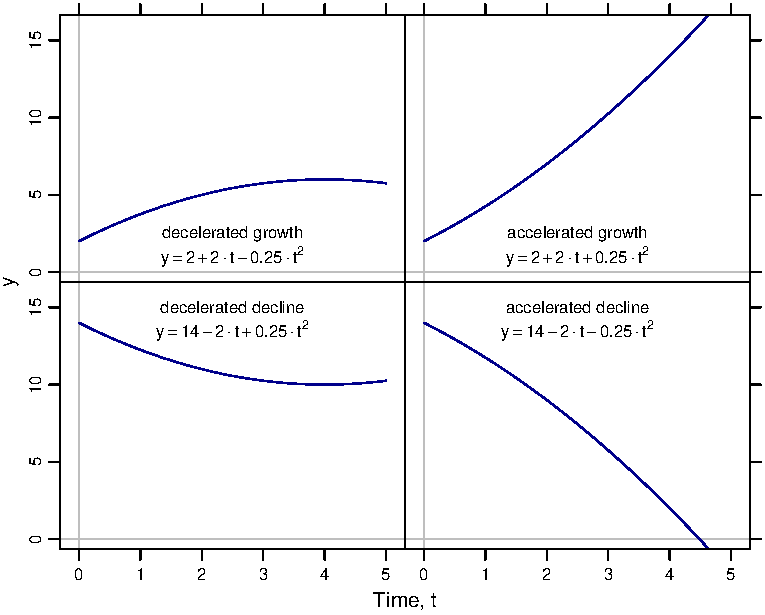
\includegraphics[width=9cm]{../figures/quad}
    \end{column}
  \end{columns}
\end{frame}

\begin{frame}{Quadratic time trends}
  \begin{itemize}
    \item Quadratic regression model
\begin{align*}
  y_{ij} &= b_{0i} + b_{1i}\,t_{ij} + b_{2i}\,t^2_{ij} + \varepsilon_{ij}\\
         &= b_{0i} + (b_{1i} + b_{2i}\,t_{ij}) t_{ij}  + \varepsilon_{ij}
\end{align*}
    \item The linear change depends on time $t$
\[
  \frac{\partial y}{\partial t} = b_{1i} + 2b_{2i} \, t
\]
    \item The intercept $t = -b_{1i}/(2 b_{2i})$ is the point in time when a
      positive (negative) trend becomes negative (postive)
  \end{itemize}
\end{frame}

\begin{frame}{Outline}
\tableofcontents
\end{frame}

\section{Depression and Imipramin}

\begin{frame}{Depression and Imipramin \citep{ReisbyGram77}}
  \begin{itemize}
    \item \citet{ReisbyGram77} studied the effect of Imipramin on 66
      inpatients treated for depression
    \item Depression was measured with the Hamilton depression rating scale
      (HDRS)
    \item Additionally, the concentration of Imipramin and its metabolite
      Desipramin was measured in their blood plasma
    \item Patients were classified into endogenous and non-endogenous
      depressed
    \item Depression was measured weekly for 6 time points; the effect of
      the antidepressant was observed starting at week 2 for four weeks
  \end{itemize}
\end{frame}




\begin{frame}{Descriptive statistics}
\begin{columns}
\begin{column}{.55\textwidth}
  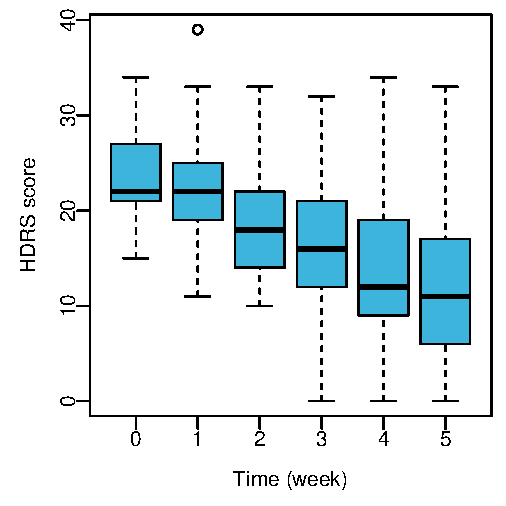
\includegraphics[scale=.8]{../figures/hdrs-box}
\end{column}
\begin{column}{.6\textwidth}
  HDRS score\\[1ex]
  {\footnotesize
\begin{tabular}{rrrrrrr}
  \hline
  $t$ & W0 & W1 & W2 & W3 & W4 & W5 \\ 
  \hline
  $M$  & 23.44 & 21.84 & 18.31 & 16.42 & 13.62 & 11.95 \\ 
  $SD$ &  4.53 & 4.70  & 5.49  & 6.42  & 6.97  & 7.22 \\ 
  $n$  & 61    & 63    & 65    & 65    & 63    & 58    \\ 
  \hline
\end{tabular}
  }

  \vspace{.5cm}
  Empirical correlation matrix of HDRS score\\[1ex]
  {\footnotesize
\begin{tabular}{rrrrrrr}
  \hline
   & W0 & W1 & W2 & W3 & W4 & W5 \\ 
  \hline
  Week 0 &   1 & .49 & .41 & .33 & .23 & .18 \\ 
  Week 1 & .49 &   1 & .49 & .41 & .31 & .22 \\ 
  Week 2 & .41 & .49 &   1 & .74 & .67 & .46 \\ 
  Week 3 & .33 & .41 & .74 &   1 & .82 & .57 \\ 
  Week 4 & .23 & .31 & .67 & .82 &   1 & .65 \\ 
  Week 5 & .18 & .22 & .46 & .57 & .65 &   1 \\ 
  \hline
\end{tabular}
  }

  \vspace{1cm}
\end{column}
\end{columns}
\end{frame}

\begin{frame}{Predictions random slope model}
  \begin{columns}
    \begin{column}{.6\textwidth}
    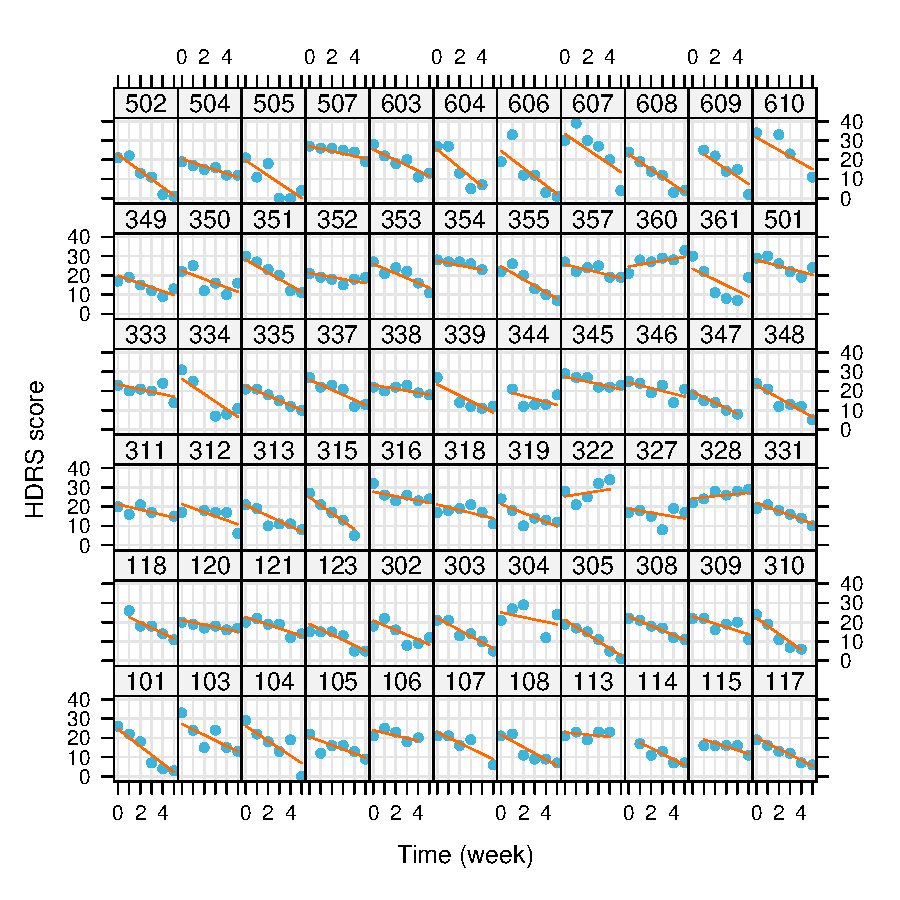
\includegraphics[scale=.5]{../figures/hdrs-ind_pred-randomslope}
    \end{column}
  \begin{column}{.4\textwidth}
  \[
    y_{ij} = \beta_0 + \beta_1 time + \upsilon_{0i} + \upsilon_{1i} time +
    \varepsilon_{ij}
  \]
with
\begin{align*}
  \begin{pmatrix} \upsilon_{0i}\\ \upsilon_{1i} \end{pmatrix} &\overset{iid}\sim
    N \left(\begin{pmatrix} 0\\ 0 \end{pmatrix}, \, \gmat{\Sigma}_\upsilon =
      \begin{pmatrix}
        \sigma^2_{\upsilon_0} & \sigma_{\upsilon_0 \upsilon_1} \\
        \sigma_{\upsilon_0 \upsilon_1} & \sigma^2_{\upsilon_1} \\
      \end{pmatrix} \right)\\
  \gvect{\varepsilon}_i &\overset{iid}\sim N(\vect{0}, \, \sigma^2 \mat{I}_{n_i})
\end{align*}
  \end{column}
\end{columns}
\end{frame}

\begin{frame}[fragile]{Model with quadratic trend}
  \begin{itemize}
    \item Model with quadratic individual and quadratic group trend
      \[
 y_{ij} = \beta_0 + \beta_1\,t_{ij} + \beta_2\,t^2_{ij} + \upsilon_{0i} +
      \upsilon_1\,t_{ij} + \upsilon_2\,t^2_{ij} + \varepsilon_{ij}
      \]
with
\begin{align*}
  \begin{pmatrix}
    \upsilon_{0i}\\
    \upsilon_{1i}\\
    \upsilon_{2i}
  \end{pmatrix} &\sim
  N \left(\begin{pmatrix}
      0\\ 0\\ 0
  \end{pmatrix}, \,
  \begin{pmatrix}
    \sigma^2_{\upsilon_0} & \sigma_{\upsilon_0 \upsilon_1} & \sigma_{\upsilon_0 \upsilon_2}\\
    \sigma_{\upsilon_0 \upsilon_1} & \sigma^2_{\upsilon_1} & \sigma_{\upsilon_1 \upsilon_2}\\
    \sigma_{\upsilon_0 \upsilon_2} & \sigma_{\upsilon_1 \upsilon_2} & \sigma^2_{\upsilon_2}\\
      \end{pmatrix} \right)
    \text{ i.i.d.} \\
  \gvect{\varepsilon}_i &\sim N(\vect{0}, \, \sigma^2 \mat{I}_{n_i})
    \text{ i.i.d.}
\end{align*}
  \end{itemize}
\vspace{-.5cm}
\end{frame}

\begin{frame}[fragile]{Depression and Imipramin}
  \begin{lstlisting}
dat      <- read.table("data/reisby.dat", header = TRUE)
dat$id   <- factor(dat$id)
dat$diag <- factor(dat$diag, levels = c("nonen", "endog"))
dat      <- na.omit(dat)     # drop missing values

# random intercept model
lme1 <- lmer(hamd ~ week + (1 | id), data = dat, REML = FALSE)

# random slope model
lme2 <- lmer(hamd ~ week + (week | id), data = dat, REML = FALSE)

# model with quadratic time trend
lme3 <- lmer(hamd ~ week + I(week^2) + (week + I(week^2) | id),
             data = dat, REML = FALSE)
  \end{lstlisting}
\end{frame}

\begin{frame}{Model predictions}
\begin{columns}
\begin{column}{6cm}
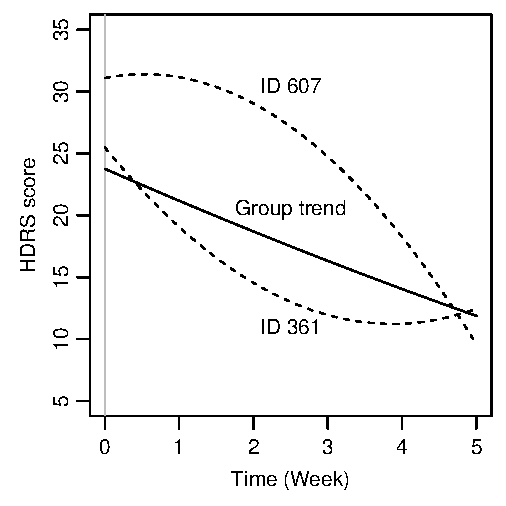
\includegraphics[width=6cm]{../figures/hdrs-quad}
\end{column}
%
\begin{column}{5cm}
  \begin{itemize}
    \item Averaged over persons an approximately linear trend is obtained,
      $\hat{\beta}_1 = -2.63$, $\hat{\beta}_2 = 0.05$
    \item Some of the predicted individual trends are strongly nonlinear
  \end{itemize}
\end{column}
\end{columns}
  \begin{itemize}
    \item Test against a model without individual quadratic trends\\[2ex]

H$_0$: $\sigma^2_{\upsilon_2} = \sigma_{\upsilon_0 \upsilon_2} =
\sigma_{\upsilon_1 \upsilon_2} = 0$ \qquad
$G^2(3) = 10.98$, $p = .012$
  \end{itemize}
\end{frame}

% \begin{frame}[fragile]{Model predictions}
%   \begin{lstlisting}
% # model without random quadratic time effect 
% lme3.0 <- lmer(hamd ~ week + I(week^2) + (week | id), dat,
%   REML = FALSE)
% 
% # model without fixed quadratic time effect 
% lme3.1 <- lmer(hamd ~ week + (week + I(week^2) | id), dat,
%   REML = FALSE)
% 
% # LRTs
% anova(lme3.0, lme3)
% anova(lme3.1, lme3)
%   \end{lstlisting}
% \end{frame}

\begin{frame}[fragile]{Model predictions}
  \begin{columns}
    \begin{column}{8cm}
      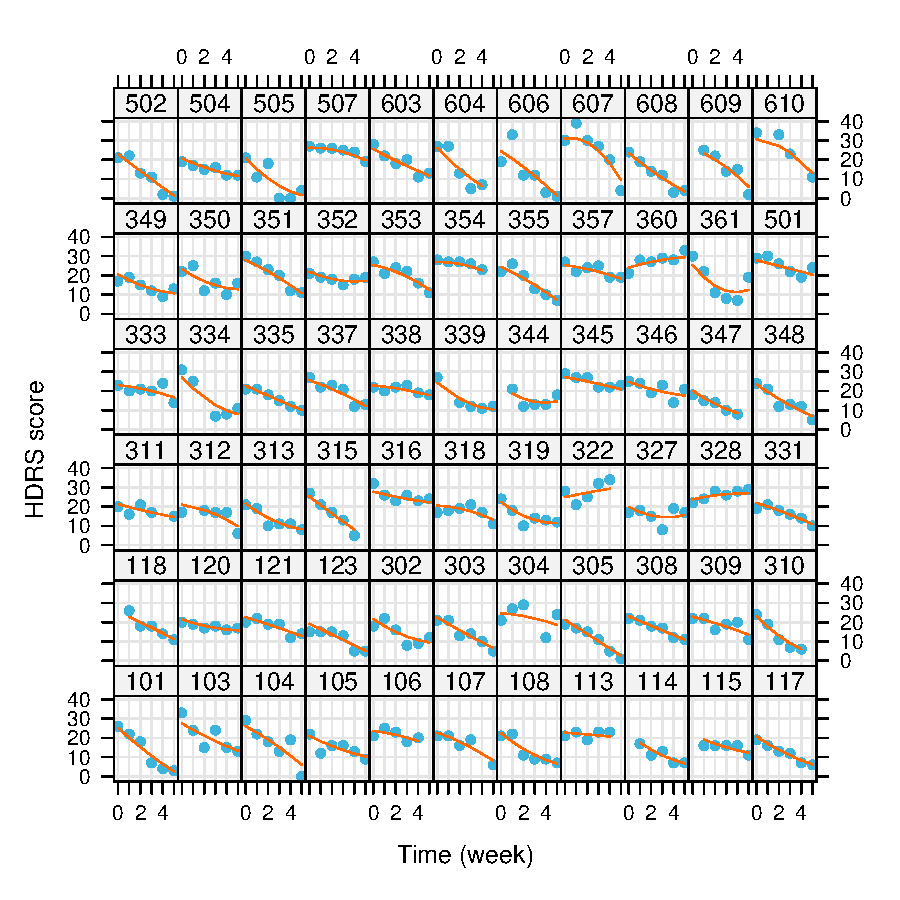
\includegraphics[scale=.5]{../figures/hdrs-ind_pred-quad}
    \end{column}
    \begin{column}{6cm}
      \begin{lstlisting}
xyplot(
  hamd + predict(lme3)
     ~ week | id,
  data = dat,
  type = c("p", "l", "g"),
  pch = 16,
  distribute.type = TRUE,
  ylab = "HDRS score",
  xlab = "Time (Week)")
      \end{lstlisting}
    \end{column}
  \end{columns}
\end{frame}

\begin{frame}[fragile]{Implied marginal covariance matrix}
Predicted
\begin{align*}
  \mat{Z}_i \gmat{\hat\Sigma}_\upsilon \mat{Z}'_i +
    \hat\sigma^2 \mat{I}_{n_i} &= 
  \begin{pmatrix}
    20.96 & 9.41 & 8.16 & 6.68 & 4.98 & 3.06 \\ 
    9.41 & 23.86 & 15.57 & 16.08 & 14.88 & 11.97 \\ 
    8.16 & 15.57 & 31.07 & 23.11 & 23.26 & 20.98 \\ 
    6.68 & 16.08 & 23.11 & 38.31 & 30.12 & 30.09 \\ 
    4.98 & 14.88 & 23.26 & 30.12 & 45.98 & 39.29 \\ 
    3.06 & 11.97 & 20.98 & 30.09 & 39.29 & 59.11
  \end{pmatrix}\\
  %
  \intertext{Observed}
  %
  \widehat{Cov}(\vect{y}_i) &=
  \begin{pmatrix}
    20.55 & 10.11 & 10.14 & 10.09 & 7.19 & 6.28 \\ 
    10.11 & 22.07 & 12.28 & 12.55 & 10.26 & 7.72 \\ 
    10.14 & 12.28 & 30.09 & 25.13 & 24.63 & 18.38 \\ 
    10.09 & 12.55 & 25.13 & 41.15 & 37.34 & 23.99 \\ 
    7.19 & 10.26 & 24.63 & 37.34 & 48.59 & 30.51 \\ 
    6.28 & 7.72 & 18.38 & 23.99 & 30.51 & 52.12 \\ 
  \end{pmatrix}\\
\end{align*}
% \vspace{-1cm}
% \begin{lstlisting}
% getVarCov(lme3, type="marginal")  # predicted cov. matrix
% 
% var.d <- crossprod(getME(lme3,"Lambdat"))
% Zt <- getME(lme3, "Zt")
% vr <- sigma(lme3)^2
% 
% var.b <- vr*(t(Zt) %*% var.d %*% Zt)
% sI <- vr * Diagonal(nrow(dat2))
% var.y <- var.b + sI
% 
% \end{lstlisting}
\end{frame}

\begin{frame}{Centering variables}
  \begin{itemize}
    \item If multiples of the time variables ($t$, $t^2$, $t^3$, etc.) are
      entered into the regression equation, multicollinearity can become a
      problem
    \item For example, $t = 0, 1, 2, 3$ and $t^2 = 0, 1, 4, 9$ correlate almost
      perfectly
    \item By centering the variables, this problem can be diminished: $(t -
      \bar{t}) = -1.5, -0.5, 0.5,  1.5$ and $(t - \bar{t})^2 = 2.25, 0.25, 0.25,
      2.25$ are uncorrelated
    \item By centering variables the interpretation of the intercept in a linear
      model changes:
  \begin{itemize}
    \item Uncentered intercepts represent the difference to the first time 
    point ($t = 0$)
    \item Centered intercepts represent the difference after half of the 
    time
  \end{itemize}
  \end{itemize}
\end{frame}

\begin{frame}[fragile]{Analysis with centered time variable}
\begin{lstlisting}
dat$week_c <- dat$week - mean(dat$week)
cor(dat$week, dat$week^2)       # 0.96
cor(dat$week_c, dat$week_c^2)   # 0.01

# random slope model
lme2c <- lmer(hamd ~ week_c + (week_c | id), data = dat, REML = FALSE)

# model with quadratic time trend
lme3c <- lmer(hamd ~ week_c + I(week_c^2) + (week_c + I(week_c^2) | id),
              data = dat, REML = FALSE)
\end{lstlisting}
  \begin{itemize}
    \item When comparing the estimated parameters, it becomes obvious that not
      only the intercept changes but the estimates for the (co)variances do as
      well
    \item Why?\pause
      ~Be sure to make an informed choice when centering your
      variables!
  \end{itemize}
  \nocite{Alday2025}
\end{frame}

\begin{frame}[fragile]{Investigating random effects structure}
  \begin{itemize}
    \item In order to get a better understanding of the necessary random effects
      it might be a good idea to take a closer look at them
    \item Two plots often used are the so-called caterpillar and shrinkage plots
    \item Play around with different models and compare how, e.\,g., the
      caterpillar plots change with and without covariances in the model!
      \pause\vspace{.5cm}
    \item We will refit our models with REML since it is better suited for
      estimating the random effects!
  \end{itemize}
\begin{lstlisting}
lme3r <- 
  lmer(hamd ~ week_c + I(week_c^2) + (week_c + I(week_c^2) | id),
       data = dat)
\end{lstlisting}
\end{frame}


\begin{frame}[fragile]{Investigating random effects structure}
  {Caterpillar plot}
  \vspace{-.4cm}
    \begin{center}
      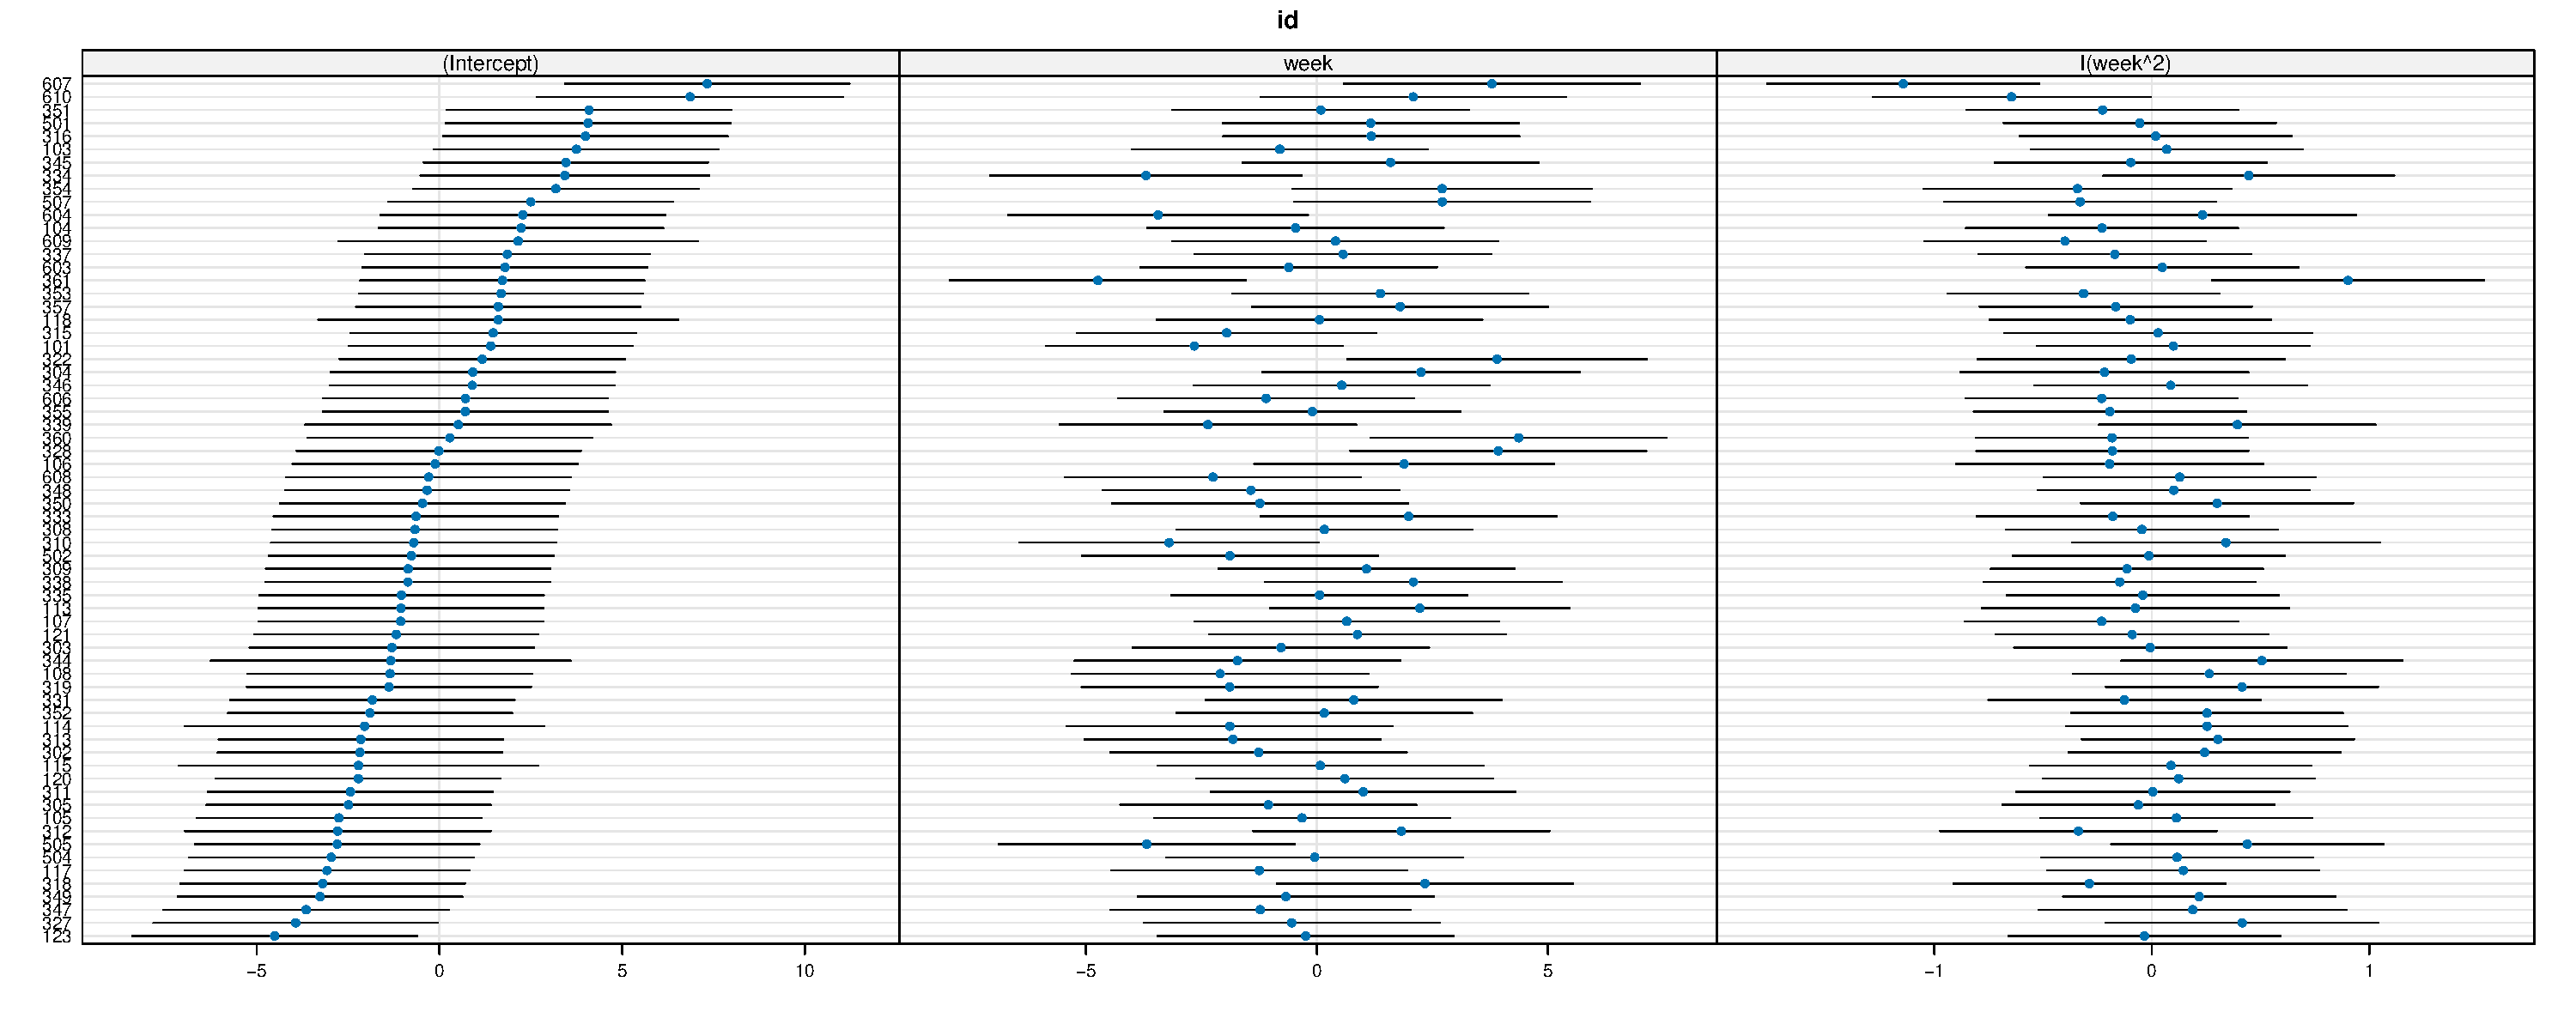
\includegraphics[scale=.25]{../figures/hdrs-caterpillar}
  \end{center}
  \vspace{-.3cm}
\begin{lstlisting}
library(lattice)
dotplot(ranef(lme3r), scales = list( x = list(relation = "free")))$id
\end{lstlisting}
\end{frame}


\begin{frame}[fragile]{Investigating random effects structure}
  {Shrinkage plots}
  \begin{columns}
    \begin{column}{.35\textwidth}
      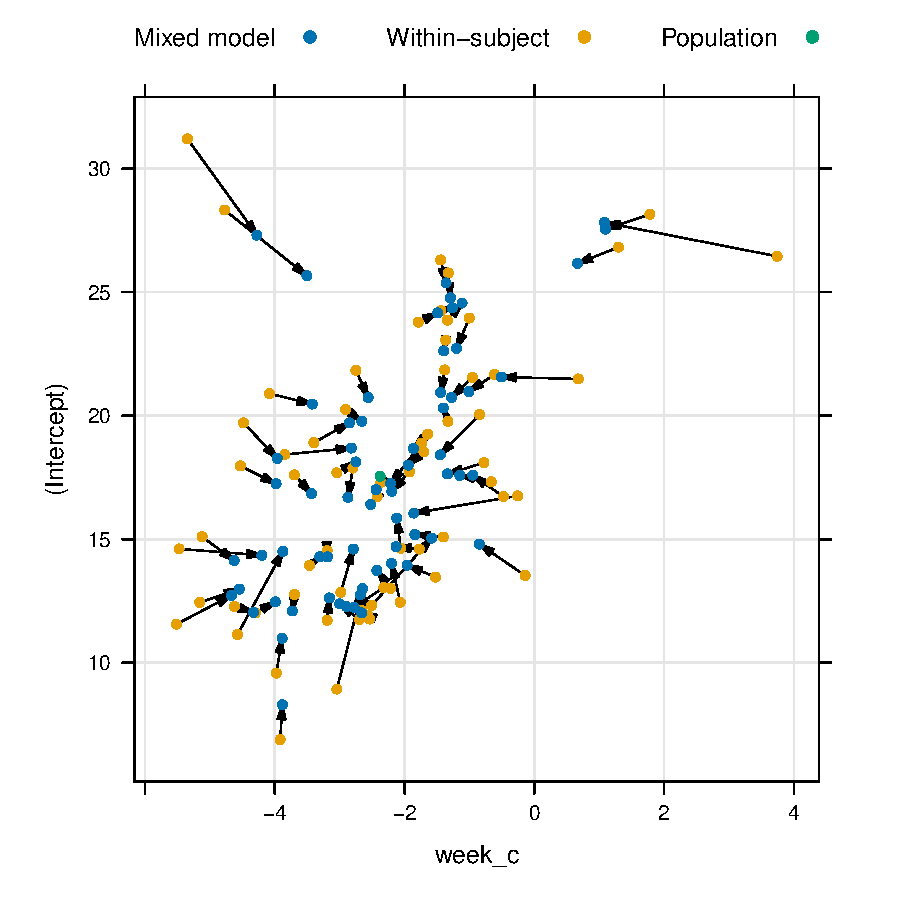
\includegraphics[scale=.35]{../figures/hdrs_shrinkage_int-week}
    \end{column}
    \begin{column}{.35\textwidth}
      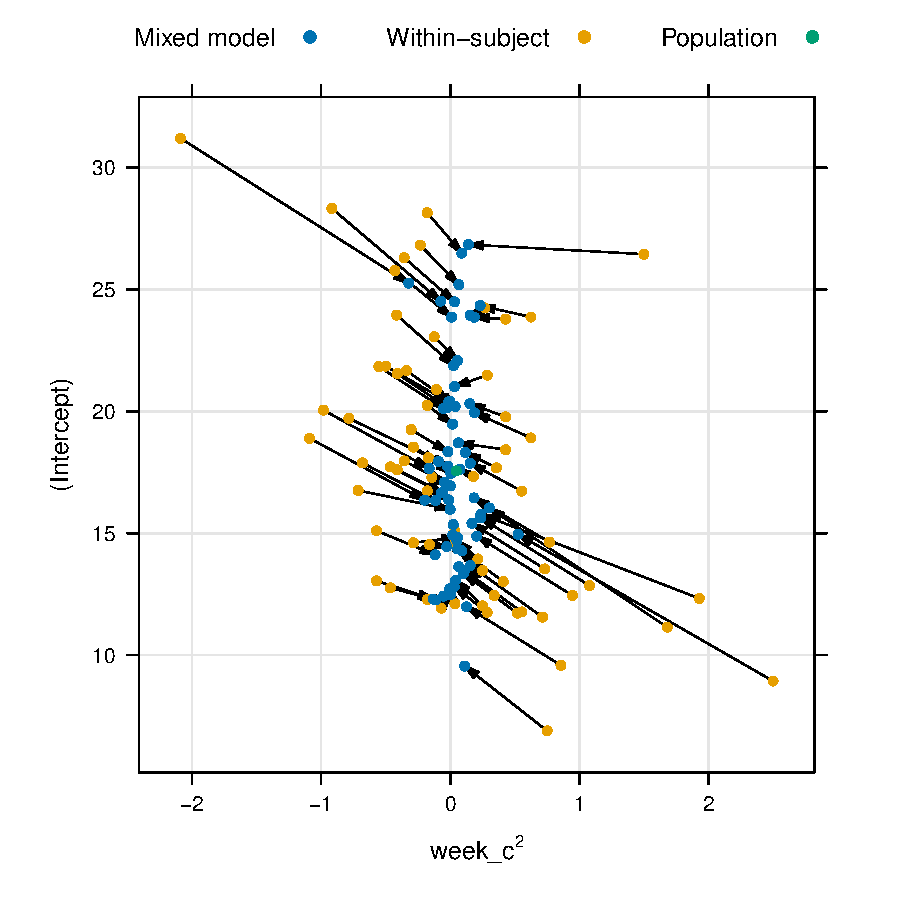
\includegraphics[scale=.35]{../figures/hdrs_shrinkage_int-weeksq}
    \end{column}
    \begin{column}{.35\textwidth}
      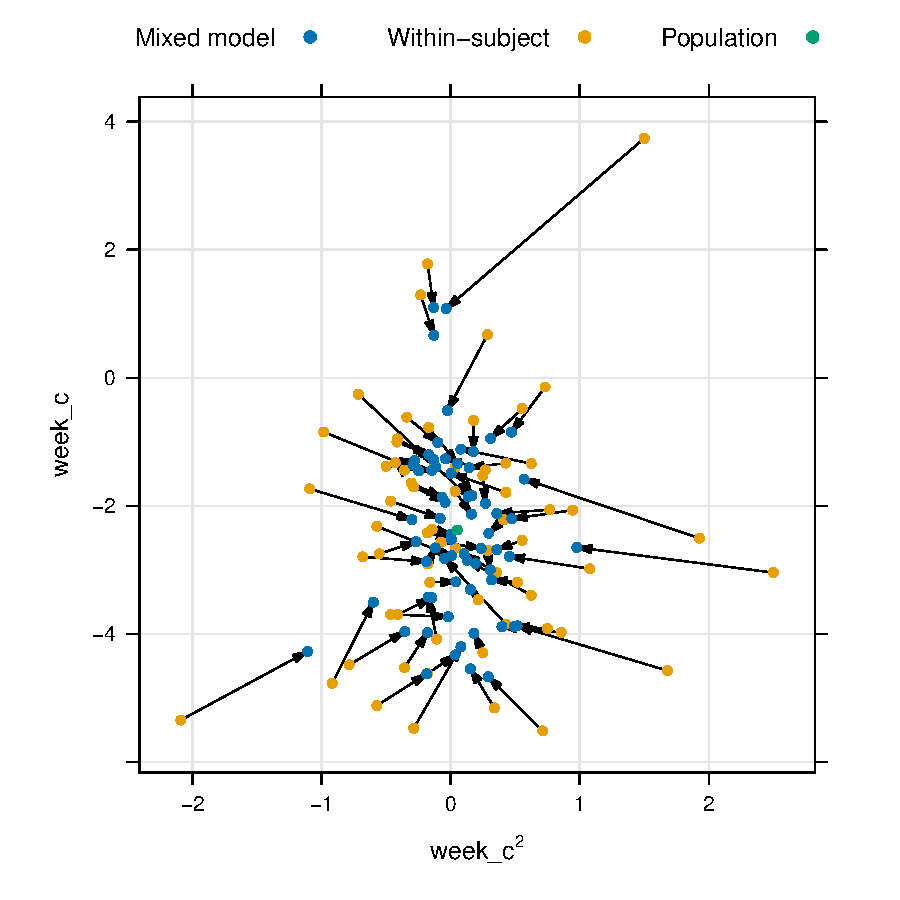
\includegraphics[scale=.35]{../figures/hdrs_shrinkage_week-weeksq}
    \end{column}
  \end{columns}
\end{frame}

\begin{frame}[fragile]{Investigating random effects structure}
  \begin{itemize}
    \item The shrinkage plots suggest that we might not need the quadratic
      effect
    \item Let us dive a little deeper and look at the profiles for the random
      effects
    \item We see that the parameter for the individual quadratic effect
      ($\sigma_3$) cannot be estimated sensibly
  \end{itemize}
\begin{lstlisting}
pm3 <- profile(lme3r, which = "theta_")

xyplot(pm3)
densityplot(log(pm3))
# --> does not show for this model
splom(pm3)
confint(pm3)
# --> parameter estimation does not seem very stable (with uncentered
# time and ML estimation it does not really work at all)
\end{lstlisting}
\end{frame}

\begin{frame}[fragile]{Investigating random effects structure}
  {Shrinkage plots}
  \begin{columns}
    \begin{column}{.35\textwidth}
      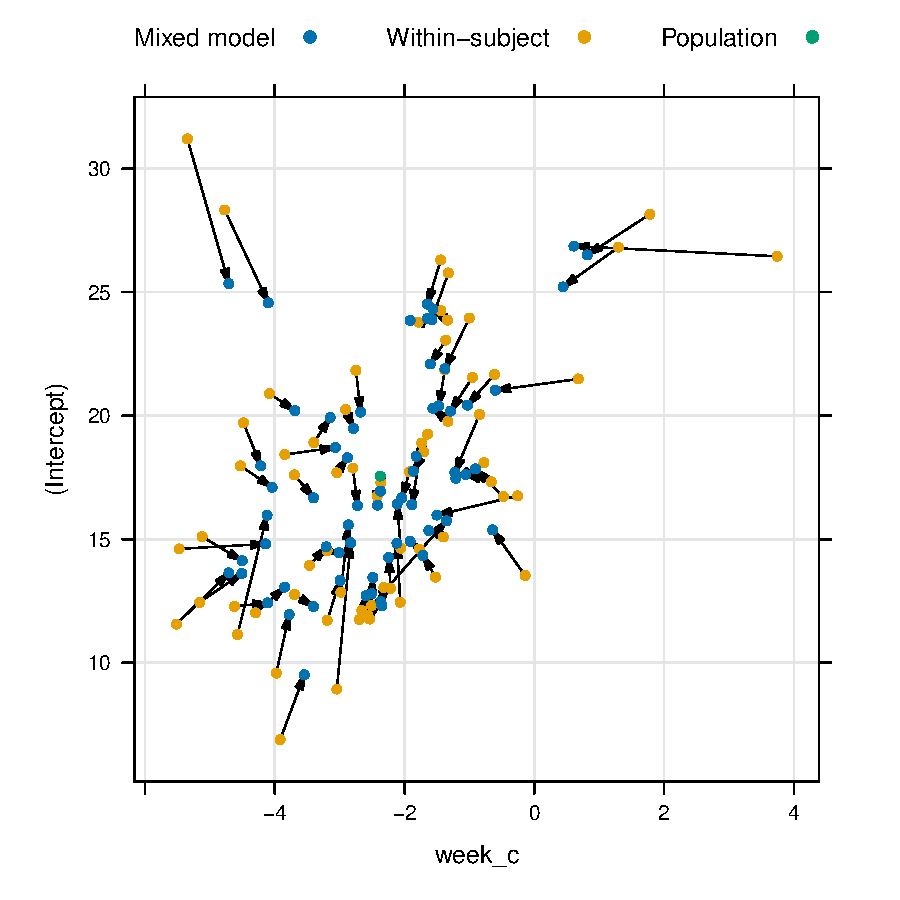
\includegraphics[scale=.35]{../figures/hdrs_shrinkage_int-week_noncorr}
    \end{column}
    \begin{column}{.35\textwidth}
      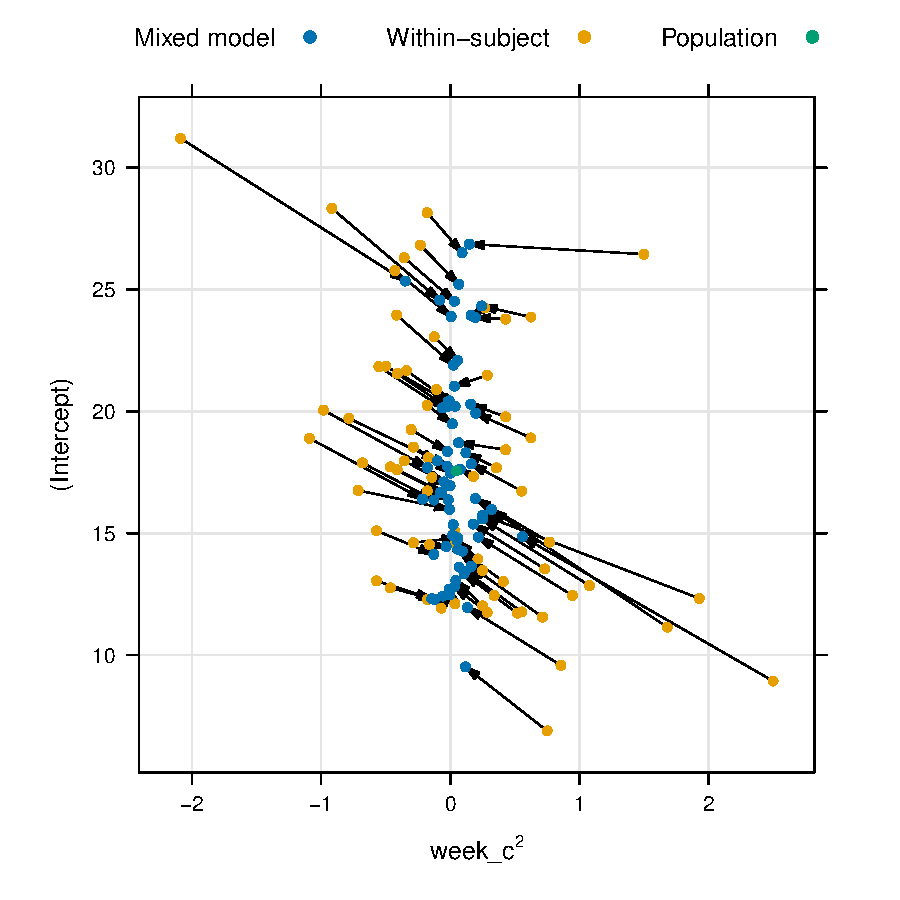
\includegraphics[scale=.35]{../figures/hdrs_shrinkage_int-weeksq_noncorr}
    \end{column}
    \begin{column}{.35\textwidth}
      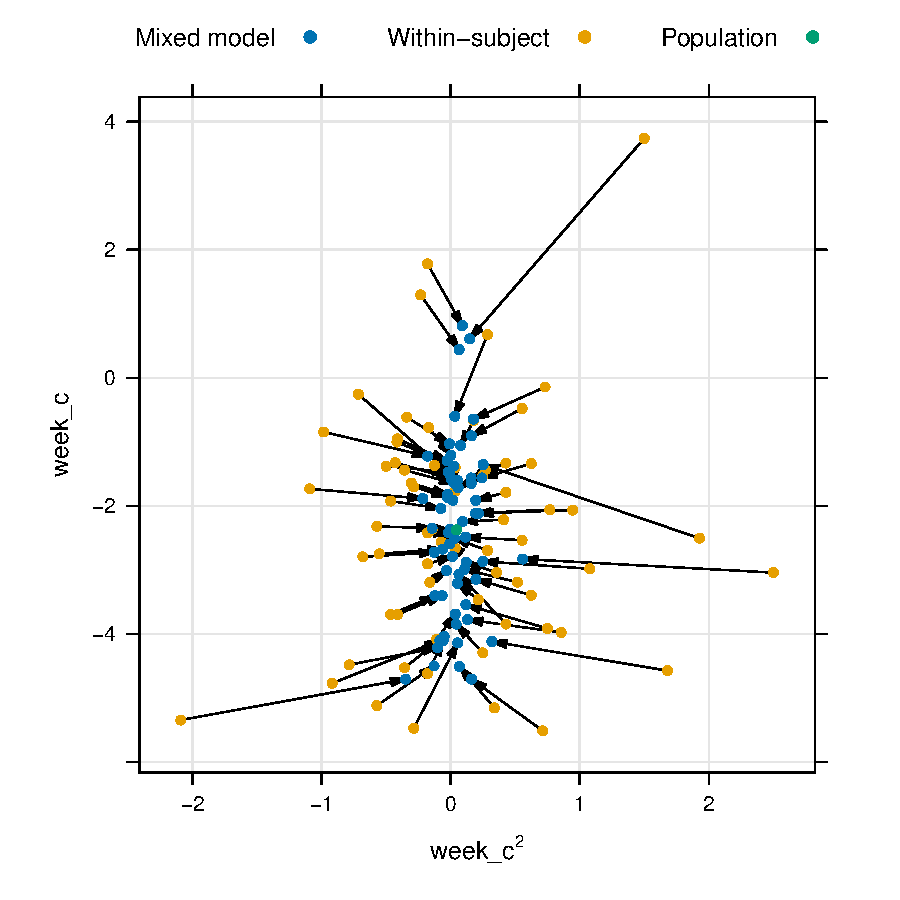
\includegraphics[scale=.35]{../figures/hdrs_shrinkage_week-weeksq_noncorr}
    \end{column}
  \end{columns}
\begin{lstlisting}
# model without covariances
lme3nc <- lmer(hamd ~ week_c + I(week_c^2) +
               (week_c + I(week_c^2) || id), data = dat)
\end{lstlisting}
\end{frame}


\begin{frame}[fragile]{Intermediate conclusions}
  \begin{itemize}
    \item After closer investigation of the random effects structure, I am not
      so sure that the story with the quadratic individual trends still holds
    \item This is only important if I want to interpret the random effects
    \item If I only include them for modeling dependency in my data, this is
      not of so much relevance
    \item In this case, I am (usually) conducting a more conservative test (more
      on this next session)
    \item Comparing models without the covariance terms also suggests that the
      quadratic time effect might not be necessary
  \end{itemize}
\begin{lstlisting}
lme2nc <- lmer(hamd ~ week_c + (week_c || id), data = dat, REML = FALSE)
lme3nc <- lmer(hamd ~ week_c + I(week_c^2) +
              (week_c + I(week_c^2) || id), data = dat, REML = FALSE)
anova(lme2nc, lme3nc)
\end{lstlisting}
\end{frame}

\begin{frame}{Higher-order polynomials}
  \begin{itemize}
    \item Nonlinear time trends can be modelled in a flexibel and parsimonious
      way by using higher-order polynomials
    \item For example, saddle or reversal points in a time trend can be
      described
    \item Polynomials have the advantage that the regression model stays linear
      in its parameters
    \item They have the disadvantage that extrapolated values can quickly be
      outside of a range that can still be interpreted in a meaningful way
  \end{itemize}
\end{frame}


\begin{frame}{Cubic time trends}
\begin{center}
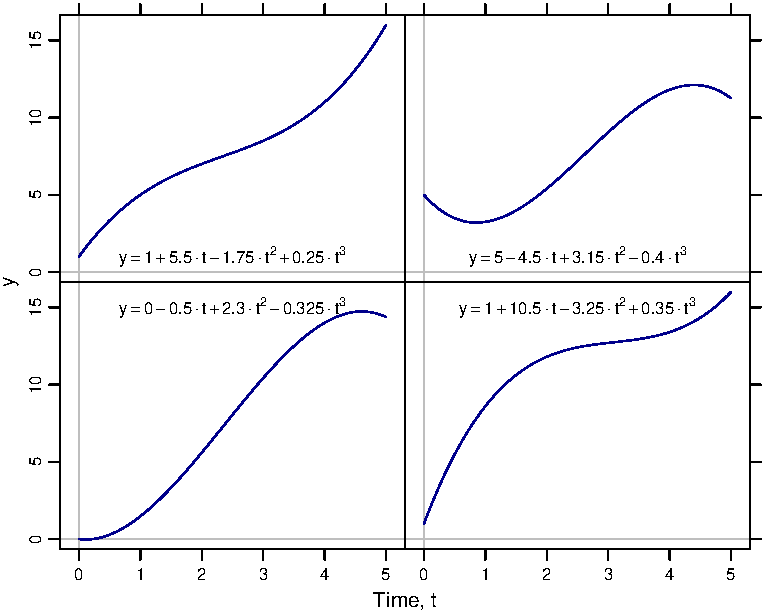
\includegraphics[width=9cm]{../figures/cubic}
\end{center}
\end{frame}


\begin{frame}{Polynomial regression: Extrapolation}
\begin{center}
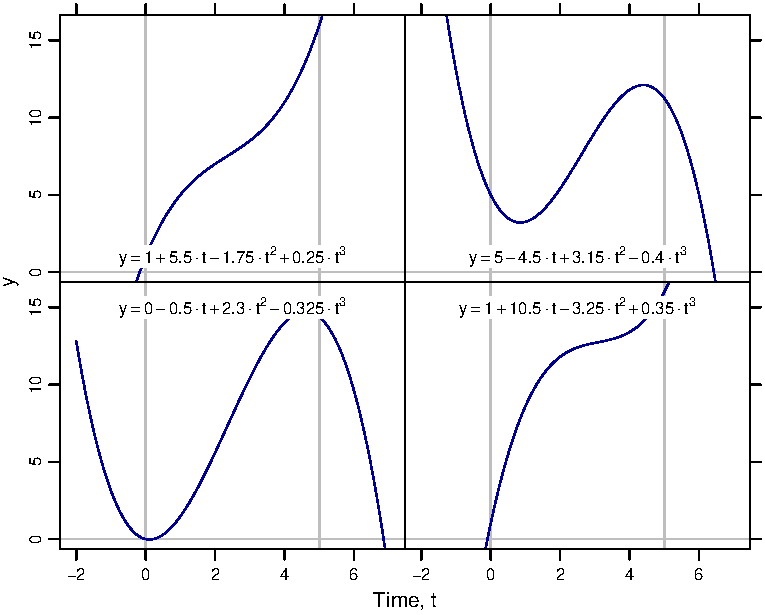
\includegraphics[width=9cm]{../figures/cubic-gone-bad}
\end{center}
\end{frame}

\section{Vocal charades}

\begin{frame}{Vocal charades \citep{Winter2016}}
This (simulated) example from linguistics is taken from \citet{Winter2016}\\[2ex]
\begin{itemize}
  \item Participants play a game of `vocal charades'
  \item At each round, a participant has to vocalize a meaning to the
  partner (e.\,g., `ugly') without using language (e.\,g., through grunting or
  hissing)
  \item The partner has to guess the meaning of the vocalization
  \item This game is played repeatedly with the finding that over time, a
  dyad converges on a set of nonlinguistic vocalizations that assure a high
  degree of intelligibility between the two participants in the dyad
\end{itemize}
\end{frame}


\begin{frame}{Example: Growth curve model}
\begin{itemize}
  \item Initially, participants may be struggling with the task and explore
  very different kinds of vocalizations
  \item Over time, they may converge on a more stable set of iconic
  vocalizations, that is vocalizations that resemble the intended referent
  (e.\,g., a high-pitched sound for `attractive' and a low-pitched sound for
  `ugly')
  \item Finally, after even more time, the dyad may conventionalize to
  idiosyncratic patterns that deviate from iconicity and become
  increasingly arbitrary
\end{itemize}
\end{frame}

\begin{frame}[fragile]{Example: Growth curve model}
  \begin{itemize}
    \item 100 observations of three variables (simulated data set)\\[2ex]
  \begin{tabular}{lp{10cm}}
      Variable & Description \\
    \hline
      \texttt{dyad} & different pairs of subjects playing the vocal charades game\\
      \texttt{t} & sequential rounds for which the vocal charades game was played \\
      \texttt{iconicity} & iconicity measure \\
     \hline
  \end{tabular}

  \vspace{.5cm}
\item For better interpretation, \texttt{t} will be centered
  \begin{lstlisting}
dat <- read.csv("data/lzw003_supplementary-data/example2_dyads.csv")
dat$dyad <- as.factor(dat$dyad)

dat$t_c <- dat$t - mean(dat$t)
  \end{lstlisting}
  \end{itemize}
\end{frame}

\begin{frame}[fragile]{Visualization of data}
  \begin{columns}
    \begin{column}{.5\textwidth}
      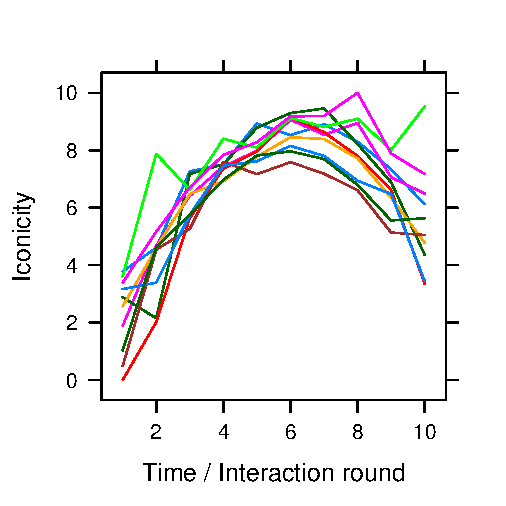
\includegraphics[scale=.8]{../figures/icon}
    \end{column}
    \begin{column}{.5\textwidth}
      \begin{lstlisting}
xyplot(
  iconicity ~ t, dat,
  groups = dyad,
  type = "l",
  xlab = "Time/Interaction round",
  ylab = "Iconicity")
      \end{lstlisting}
    \end{column}
  \end{columns}
\end{frame}

\begin{frame}[fragile]{Mixed-effects model with quadratic trend}
  \begin{itemize}
    \item We will now consider a model with uncorrelated random effects
  \[
    y_{ij} = \beta_0 + \beta_1 t_{ij} + \beta_2 t^2_{ij} + \upsilon_{0i} +
    \upsilon_{1i} t_{ij} + \upsilon_{2i} t^2_{ij} + \varepsilon_{ij}
  \]
with
\begin{align*}
  \begin{pmatrix}
    \upsilon_{0i}\\
    \upsilon_{1i}\\
    \upsilon_{2i}
  \end{pmatrix} &\sim
  N \left(\begin{pmatrix}
      0\\ 0\\ 0
  \end{pmatrix}, \,
  \begin{pmatrix}
    \sigma^2_{\upsilon_0} & 0 & 0\\
    0 & \sigma^2_{\upsilon_1} & 0\\
    0 & 0 & \sigma^2_{\upsilon_2}\\
      \end{pmatrix} \right)
    \text{ i.i.d.} \\
  \gvect{\varepsilon}_i &\sim N(\vect{0}, \, \sigma^2 \mat{I}_{n_i})
    \text{ i.i.d.}
\end{align*}
\vspace{-.8cm}
  \item This model is fitted by
\begin{lstlisting}
gcm1 <- lmer(iconicity ~ t_c + I(t_c^2) +
  (1 | dyad) + (0 + t_c | dyad) + (0 + I(t_c^2) | dyad),
  data = dat, REML = FALSE)
\end{lstlisting}
  \end{itemize}
\end{frame}

\begin{frame}[fragile]{Visualization of model predictions}
  \begin{columns}
    \begin{column}{.5\textwidth}
      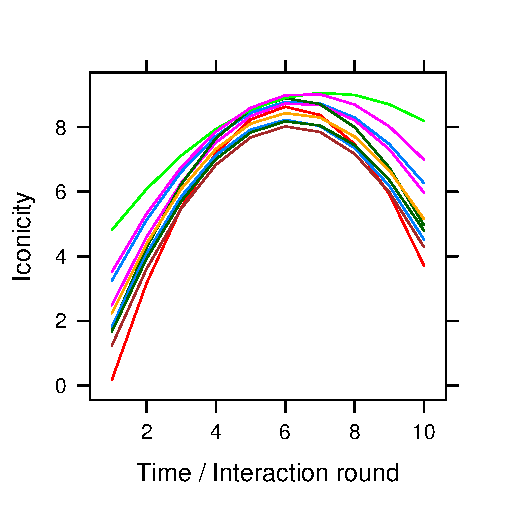
\includegraphics[scale=.8]{../figures/icon-pre}
    \end{column}
    \begin{column}{.5\textwidth}
      \begin{lstlisting}
xyplot(
  predict(gcm1) ~ t, dat,
  groups = dyad,
  type = "l",
  xlab = "Time/Interaction round",
  ylab = "Iconicity")
      \end{lstlisting}
    \end{column}
  \end{columns}
\end{frame}

% \begin{frame}[fragile]{ML estimates of parameters}
% \begin{lstlisting}
% ...
% Random effects:
%  Groups   Name        Variance Std.Dev.
%  dyad     (Intercept) 0.152845 0.39095 
%  dyad.1   t_c         0.002595 0.05094 
%  dyad.2   I(t_c^2)    0.003504 0.05920 
%  Residual             0.429691 0.65551 
% Number of obs: 100, groups:  dyad, 10
% 
% Fixed effects:
%             Estimate Std. Error t value
% (Intercept)  8.45761    0.15849   53.36
% t_c          0.35475    0.02793   12.70
% I(t_c^2)    -0.22558    0.02078  -10.86
% ...
% \end{lstlisting}
% \end{frame}

\begin{frame}{Interpretation of results}
\begin{itemize}
  \item There are now two slopes, one for the effect of linear time ($t_c$,
  $\beta_1 = 0.35$) and one for the effect of quadratic time ($t_c^2$,
  $\beta_2 = -0.23$), both of which are allowed to differ by dyad
  ($\sigma_{\upsilon_{1i}} = 0.05$ and $\sigma_{\upsilon_{2i}} = 0.06$)
  \item The negative value for the quadratic term indicates the inverse
  U-shape
  \item The point of reversal is $t = \bar t + \frac{-\hat\beta_1}{2\cdot\hat\beta_2} =
  5.5 + \frac{-.35}{2\cdot(-.22)} = 6.29$ \item The model assumes that the
  random intercept and slopes are all
  uncorrelated
\end{itemize}
\end{frame}

\begin{frame}[fragile]{Check model assumptions}
\begin{lstlisting}
hist(residuals(gcm1))   # o.k.
qqmath(gcm1)            # o.k.
plot(gcm1)              # o.k.
\end{lstlisting}
    \vspace{-.5cm}
  \begin{columns}
    \begin{column}{.5\textwidth}
      \begin{center}
      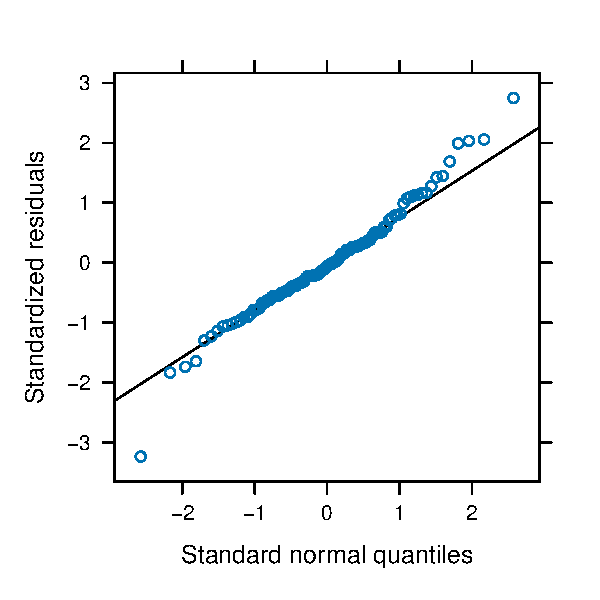
\includegraphics[scale=.55]{../figures/icon-qqplot}
      \end{center}
    \end{column}
    \begin{column}{.5\textwidth}
      \begin{center}
      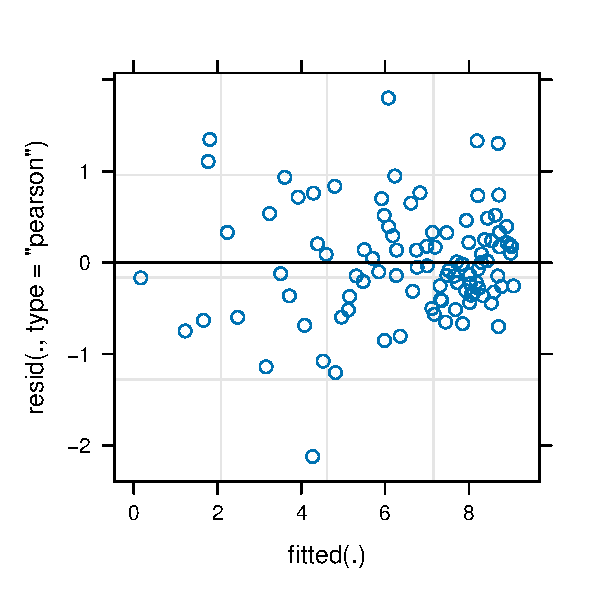
\includegraphics[scale=.55]{../figures/icon-residplot}
      \end{center}
    \end{column}
  \end{columns}
\end{frame}

% \begin{frame}{Plots from the article}
% \begin{center}
% 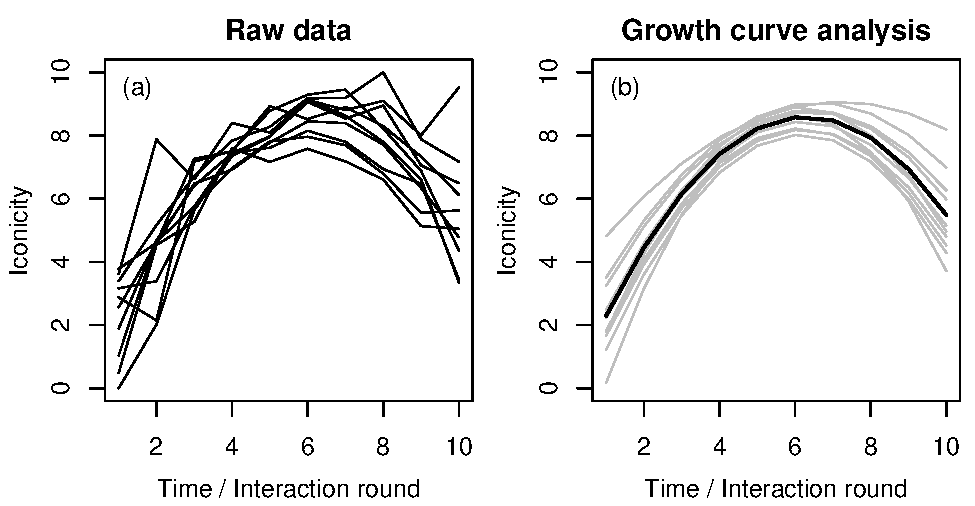
\includegraphics[scale=.8]{../figures/icon-both}
% \end{center}
% \end{frame}

\begin{frame}[fragile]{}
    \footnotesize
  \begin{block}{Exercise\footnote{Inspired by
    \url{https://embraceuncertaintybook.com/longitudinal.html\#the-elstongrizzle-data}}}
    \begin{itemize}
      \item Load the data set \texttt{elstongrizzle.dat} into R; data are from a
        dental study measuring the lengths of the ramus of the mandible (mm) in
        20 boys at 8, 8.5, 9, and 9.5 years of age
      \item Plot the individual data points for each subject either as a
        spaghetti plot and/or as a panel plot
      \item Fit a random slope model to the data; how would you interpret the
        correlation parameter in the model?
      \item Recenter your time variable, so that zero means ``8 years old''
      \item Refit your random slope model; try to explain why and how the
        correlation parameter changes
      \item Look at the caterpillar plots for the random slope model with and
        without recentered time variable; why do they look different?
      \item Create a shrinkage plot plotting the individual intercept as a
        function of the individual slopes
      \item Add individual and quadratic time effects to your model; test this
        model against the random slope model
      \item Look at the profiles for the random effects for the quadratic model;
        what would you conclude?
    \end{itemize}
  \end{block}
\end{frame}

\appendix

%\begin{frame}[allowframebreaks]{References}
\begin{frame}{References}
%\renewcommand{\bibfont}{\footnotesize}
  \printbibliography
  \vfill
\end{frame}
 
\end{document}

